\section{Performance Evaluation}
\label{performance_analysis}

This section reports the performance-comparison results supplied with the conference source manuscript \cite{gupta2025efficient}. The evaluation compares four scheduling approaches: exact Mixed-Integer Linear Programming (MILP), Greedy scheduling, randomized Relaxation, and a Metaheuristic based on a genetic algorithm. The charts are retained as reported simulation results. They provide four complementary views of scheduler behaviour: deadline flexibility, federated resource scale, workflow scale, and workflow-node failure resilience. No additional measured energy, cost, throughput, or cloud/HPC results are introduced because raw trace data for those quantities were not supplied.

\subsection{Simulation Scenario and Evaluation Dimensions}

The source study uses a custom simulation framework for DAG workflows on heterogeneous federated fog resources. Each scenario specifies the task execution characteristics, dependency relationships, deadline constraints, resource eligibility, and bandwidth-sensitive communication delay. The scientific-workflow interpretation developed in this paper treats these inputs as a portable workflow and resource descriptor. Thus, the results can be read as a focused evaluation of the latency-sensitive federated-fog tier of a larger Compute Continuum.

The four compared methods have distinct decision styles. MILP seeks a global optimum for the modelled instance. Relaxation first solves a continuous approximation and then converts the result into a discrete allocation. Greedy scheduling makes local decisions using task priority, earliest start time, and data-transfer delay. The Metaheuristic searches a larger assignment space using genetic operators. The methods are compared against the same reported workflow and resource conditions.

\begin{table*}[t]
\centering
\caption{Performance-comparison dimensions represented by the supplied simulation figures.}
\label{tab:performance_dimensions}
\small
\begin{tabular}{p{0.20\textwidth}p{0.21\textwidth}p{0.27\textwidth}p{0.22\textwidth}}
\toprule
\textbf{Dimension} & \textbf{Scenario range} & \textbf{Question addressed} & \textbf{Compute-Continuum relevance} \\
\midrule
Deadline flexibility & Slack factor $\alpha$ from 1.0 to 2.0 & How does a larger deadline budget affect the reported average-accuracy score? & Resource-aware scheduling under variable latency budgets. \\
\addlinespace
Federated resource scale & 2, 4, 6, 8, and 10 fog nodes & How does access to more nearby resources change the reported average-accuracy score? & Scalability across distributed execution resources. \\
\addlinespace
Workflow scale & 10, 100, and 1000 DAG nodes & Which algorithms retain performance as the task graph grows? & Large-scale scientific workflow orchestration. \\
\addlinespace
Failure resilience & 0\% to 50\% workflow-node failure rate & How does the reported average-accuracy score change under failures? & Adaptive execution and resilience. \\
\bottomrule
\end{tabular}
\end{table*}

\subsection{Deadline Flexibility}

Figure~\ref{fig:perf_slack_accuracy} compares the reported average-accuracy score as the slack factor $\alpha$ increases. The supplied plot shows that all approaches benefit from a less restrictive deadline. The MILP curve is the global optimisation reference; Relaxation and the Metaheuristic track it more closely than the Greedy baseline over the larger slack settings. This result is consistent with the purpose of approximate execution: when a workflow has a short deadline, the scheduler may need to reduce execution fractions or make a faster local placement decision, whereas a larger time budget permits higher-fidelity task execution.


For a Compute-Continuum orchestrator, slack is an actionable policy input. A latency-critical control loop may assign a small slack factor and favour a nearby fog placement. A less urgent simulation or post-processing stage can tolerate a larger slack factor and can use a broader candidate-resource set. The figure therefore does not merely represent a tuning parameter; it illustrates the trade-off between timeliness and achieved computational fidelity. From an orchestration standpoint, this characterises how much scheduling flexibility a Compute-Continuum orchestrator must reserve to guarantee workflow-level deadline adherence under bandwidth constraints, and therefore how conservatively a deadline should be advertised to a workflow submitter.

\subsection{Federated Resource Scale}

Figure~\ref{fig:perf_nodes_accuracy} evaluates the effect of increasing the number of fog nodes. The reported average-accuracy score rises as additional resources become available. The result demonstrates the value of federation: a workload that cannot achieve a high-accuracy schedule in an isolated local environment can benefit from neighbouring resources when the data-transfer cost remains acceptable. The comparison also shows that the scheduling policy matters even when more resources are available; access to capacity alone does not ensure that dependencies and communication paths are used efficiently.


Within the Compute Continuum, this result motivates a resource-discovery policy that exposes nearby, compatible resources to the scheduler. Adding an edge, fog, cloud, or HPC resource to the candidate set should be conditional on eligibility and estimated communication delay. The model captures this condition through $P_{ia}$ and $c_{ji}^{ba}$, ensuring that a remote resource is selected only when its expected benefit outweighs transfer overhead. Read as an orchestration result, this indicates how orchestration quality scales as the federated tier of the continuum grows, and gives a basis for deciding when adding a resource to the candidate set improves attainable accuracy rather than merely enlarging the search space.

\subsection{Workflow-Scale Comparison}

Figure~\ref{fig:perf_task_size_accuracy} compares the reported average-accuracy score for DAGs containing 10, 100, and 1000 tasks. The chart supports the scalability motivation for the retained approximation and metaheuristic methods. MILP provides a high-quality reference for smaller instances, but becomes less practical as the number of scheduling decisions grows. Relaxation and the Metaheuristic retain higher reported scores than the Greedy baseline at the larger workflow sizes, while the Greedy method offers a lower-complexity alternative when a rapid response is the dominant requirement.


The workflow-scale result is relevant to eScience pipelines that combine many data transformations, simulation stages, and machine-learning tasks. It suggests a tiered orchestration strategy: use exact optimisation to analyse small or stable subgraphs and use relaxation or metaheuristic methods for large, dynamic, or time-constrained subgraphs. This strategy retains the same task and data semantics while adapting the optimisation effort to the operational scale. It also establishes which scheduling method an orchestrator should select as workflow complexity grows, and is the empirical basis for the selection policy in Table~\ref{tab:orchestration_policy}.

\subsection{Failure-Resilience Comparison}

Figure~\ref{fig:perf_failure_accuracy} adds the resilience dimension required by Compute-Continuum workflows. The reported average-accuracy score decreases as the workflow-node failure rate rises from 0\% to 50\%. Across the plotted scenarios, the Relaxation and Metaheuristic approaches retain higher scores than the Greedy baseline, while MILP remains the high-quality reference. The figure does not evaluate a specific recovery protocol; rather, it quantifies the scheduling consequence of increasing the failure pressure under the supplied simulation assumptions.


For deployment, a failure detector or orchestration layer can react to a failed node by removing it from the eligible resource set and re-running the selected scheduler with the current resource graph. The scheduling model already provides the relevant input for such a decision: remaining resources, task dependencies, data locations, bandwidth, and deadline budget. An end-to-end evaluation of recovery time, state replication, and security policy is left for future work because those measurements are outside the supplied result set. Interpreted at the orchestration layer, the trend bounds the accuracy an operator can expect to retain across a replanning cycle, and motivates the adaptive execution loop of Section~\ref{sec:orchestration} rather than a single up-front placement.

\subsection{Cross-Dimension Discussion}

Table~\ref{tab:performance_dimensions} and Figures~\ref{fig:perf_slack_accuracy}--\ref{fig:perf_failure_accuracy} establish a consistent pattern. Exact optimisation is valuable as an upper-quality reference, but its computational burden limits routine use for large and dynamic workflows. Relaxation provides an attractive balance between solution quality and scalability. The Metaheuristic provides a broader search mechanism that can retain high reported accuracy under resource and workflow variation. The Greedy method remains useful when an orchestrator must make a quick local decision, though its reported accuracy is lower in the more constrained and failure-prone scenarios.

These conclusions are appropriately scoped for the supplied simulation plots. They show comparative scheduling behaviour under the specified inputs; they do not establish universal superiority across all application domains, hardware architectures, or data-governance policies. A reproducible artifact package, as described in Section~\ref{sec:reproducibility}, is needed to reproduce the plots, test additional scenarios, and evaluate real Compute-Continuum deployments.

\begin{figure*}[t]
\centering
\begin{subfigure}[t]{0.48\textwidth}
\centering
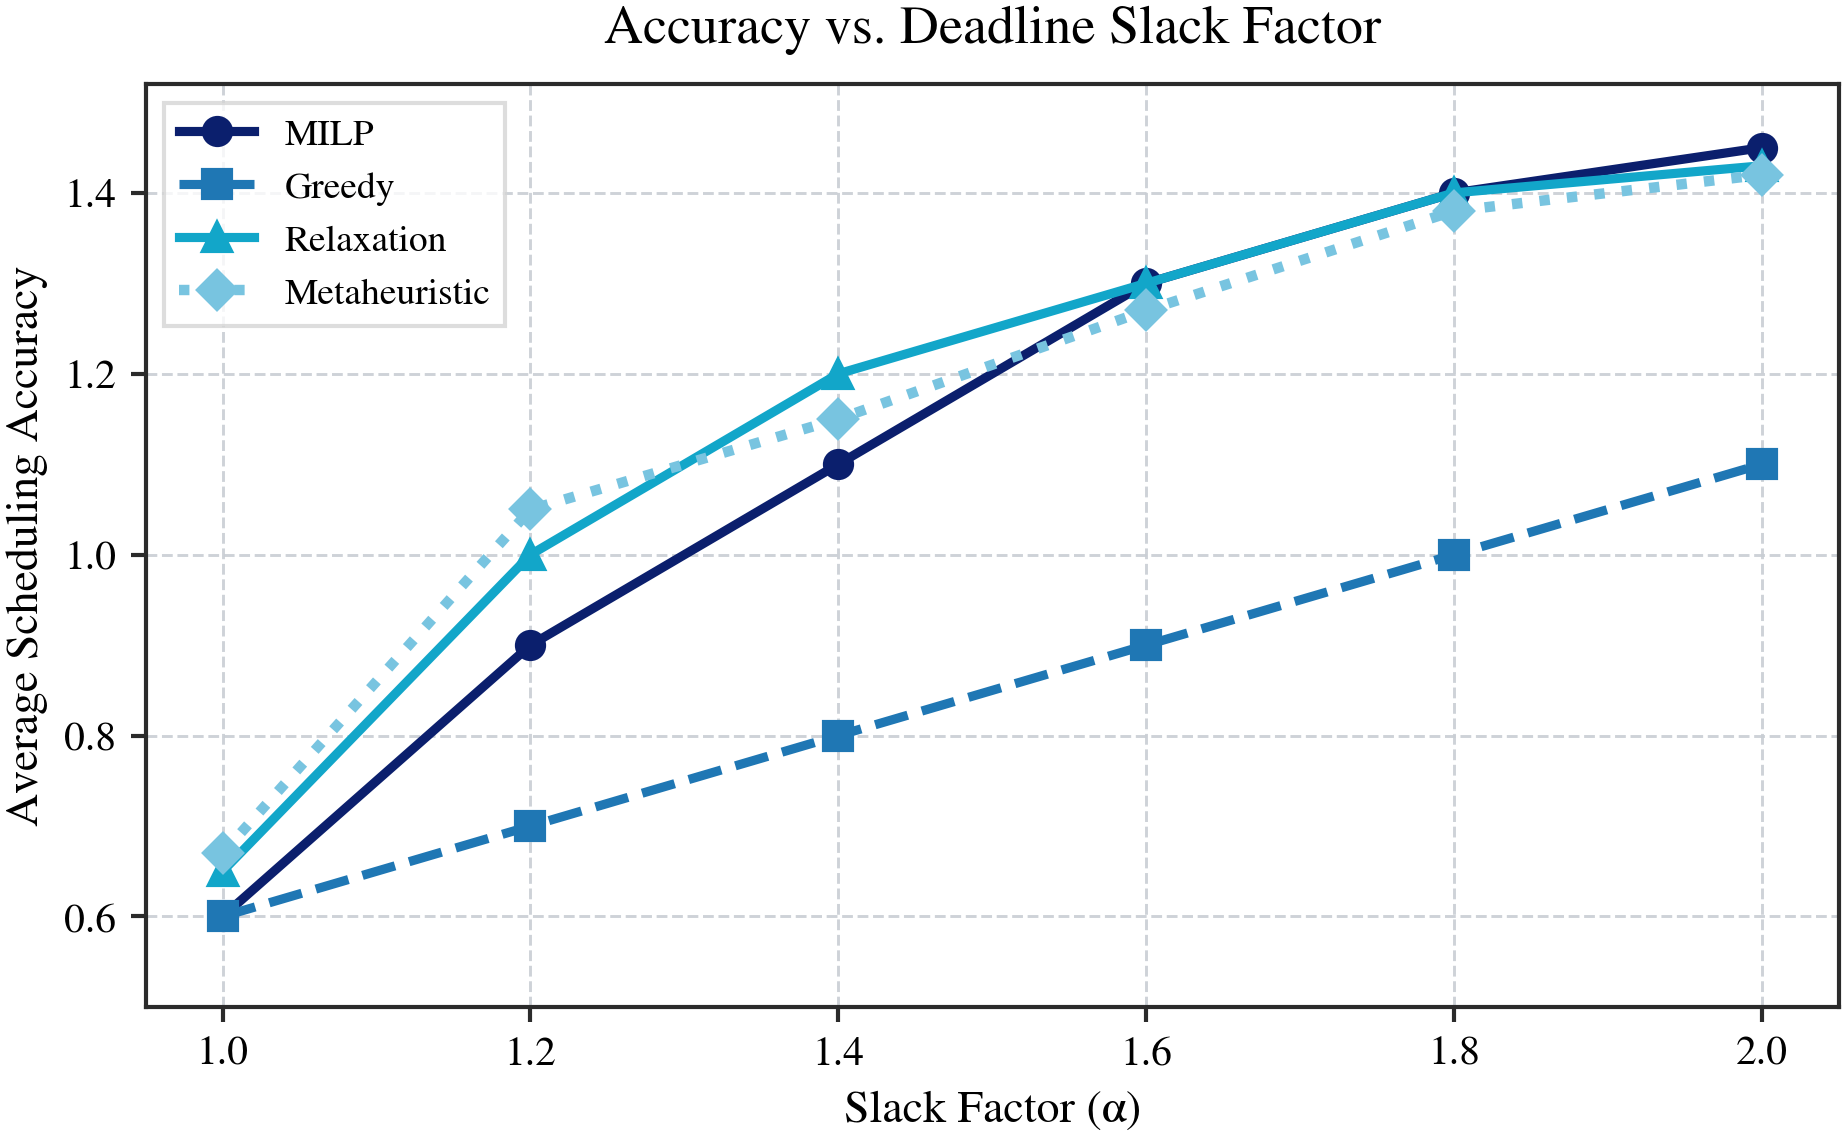
\includegraphics[width=\linewidth]{Figures/perf_slack_accuracy.png}
\caption{Reported average-accuracy comparison under slack-factor variation.}
\label{fig:perf_slack_accuracy}
\end{subfigure}\hfill
\begin{subfigure}[t]{0.48\textwidth}
\centering
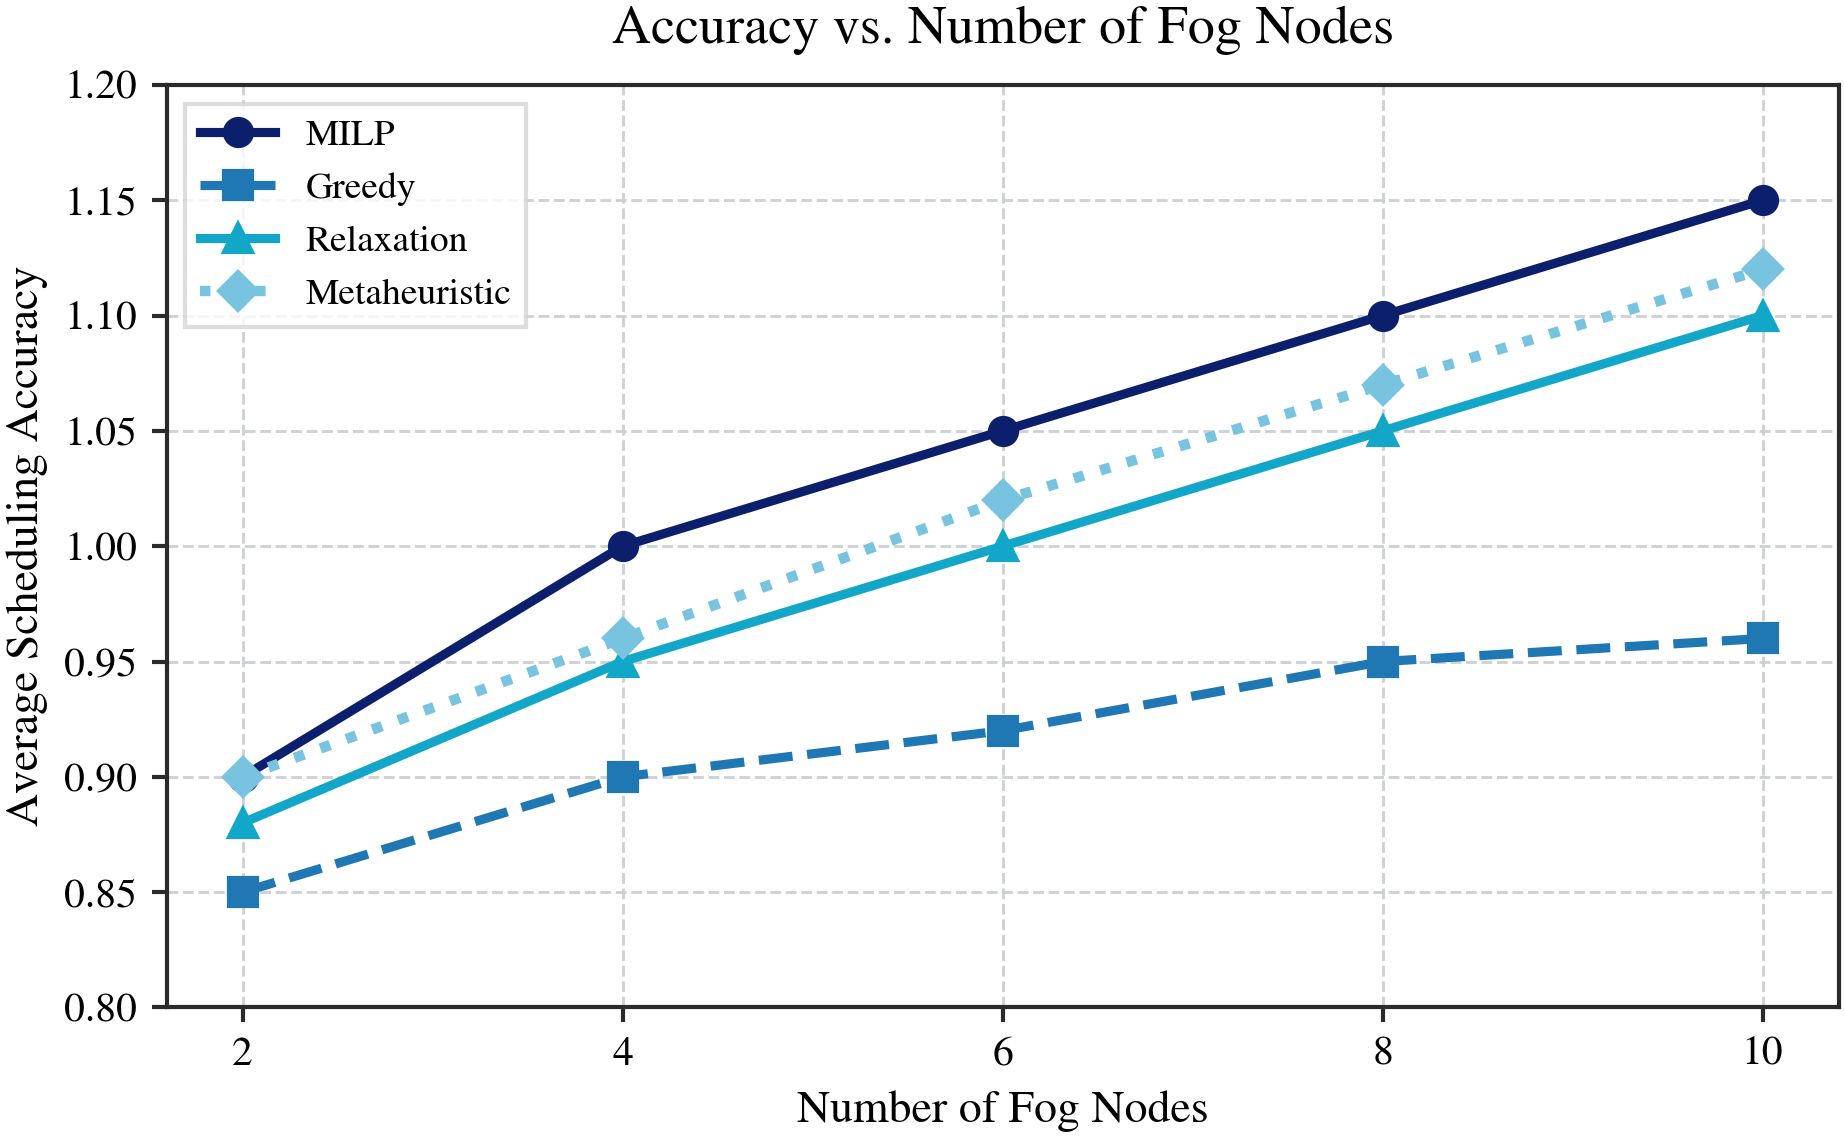
\includegraphics[width=\linewidth]{Figures/perf_nodes_accuracy.png}
\caption{Reported average-accuracy comparison as the number of federated fog nodes increases from 2 to 10.}
\label{fig:perf_nodes_accuracy}
\end{subfigure}

\vspace{1mm}
\begin{subfigure}[t]{0.48\textwidth}
\centering
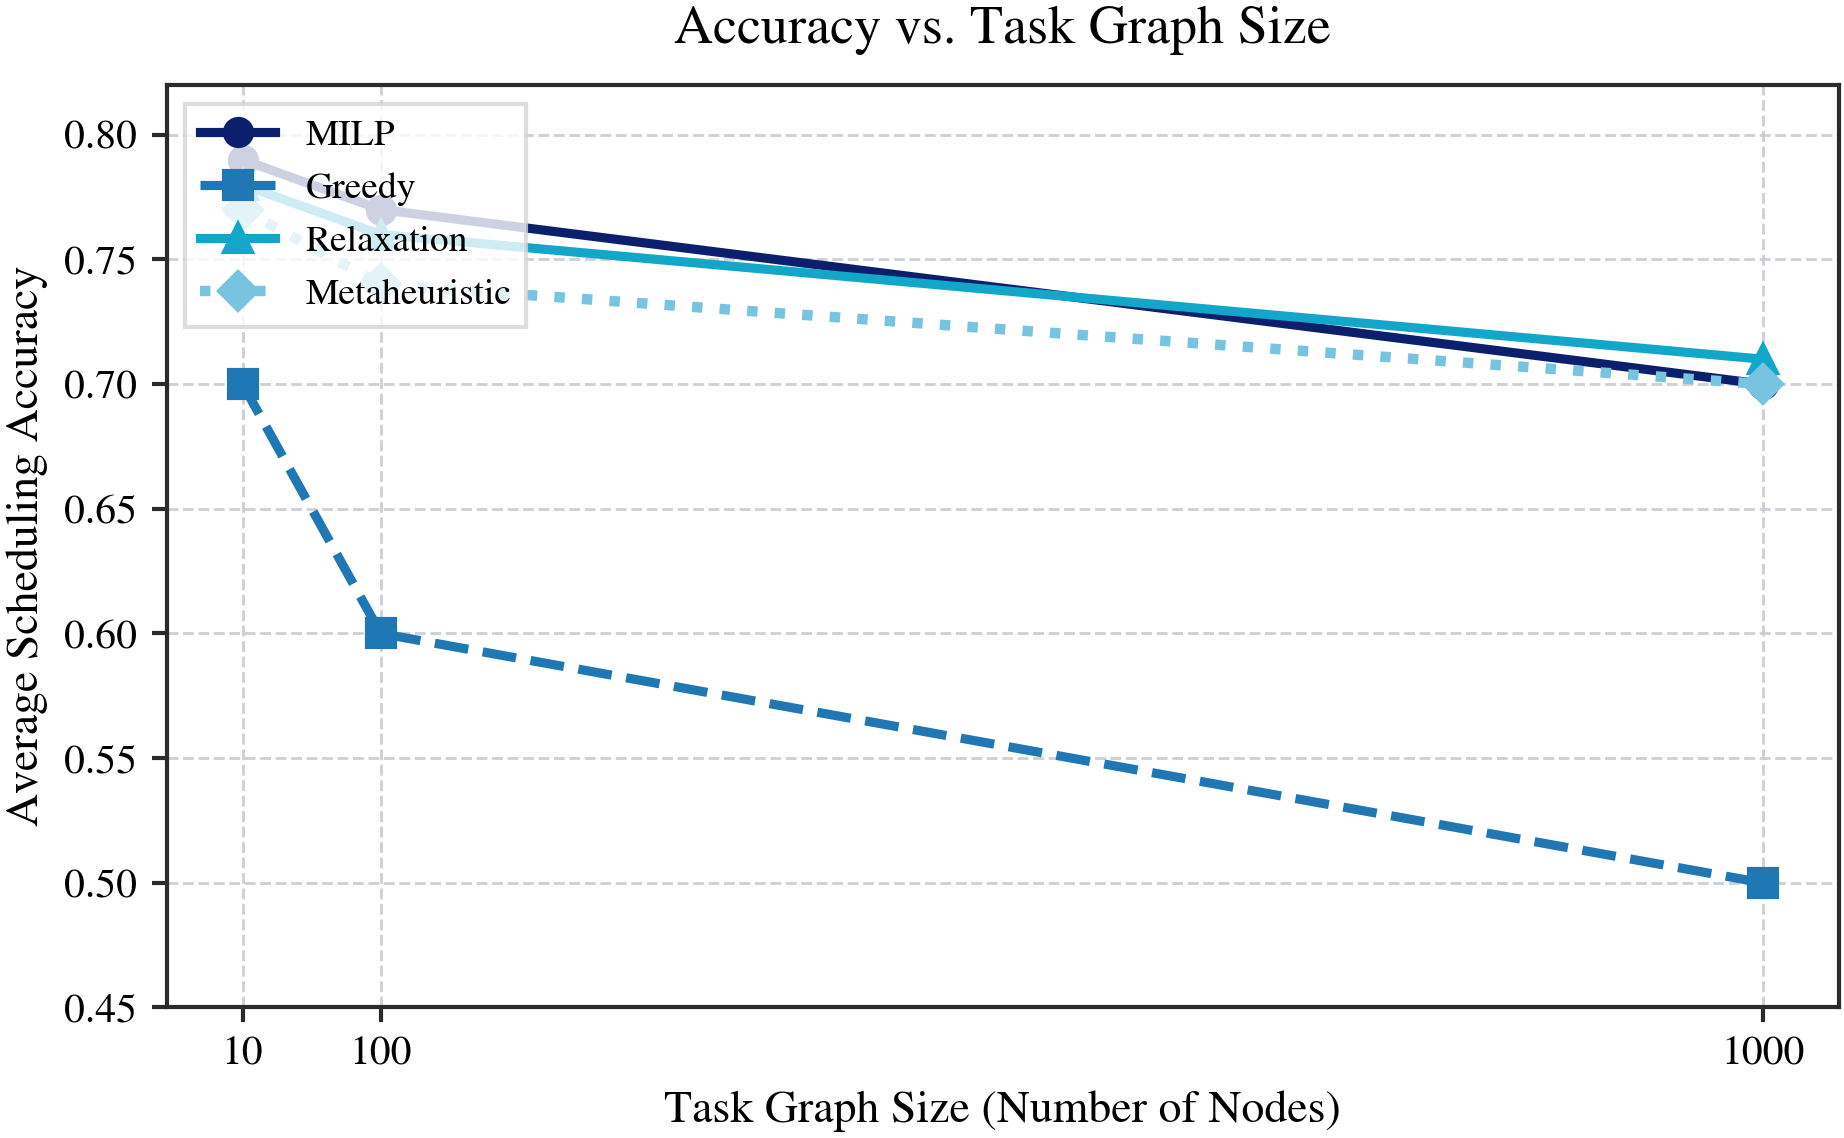
\includegraphics[width=\linewidth]{Figures/perf_task_size_accuracy.png}
\caption{Reported average-accuracy comparison as the DAG scale increases from 10 to 1000 tasks.}
\label{fig:perf_task_size_accuracy}
\end{subfigure}\hfill
\begin{subfigure}[t]{0.48\textwidth}
\centering
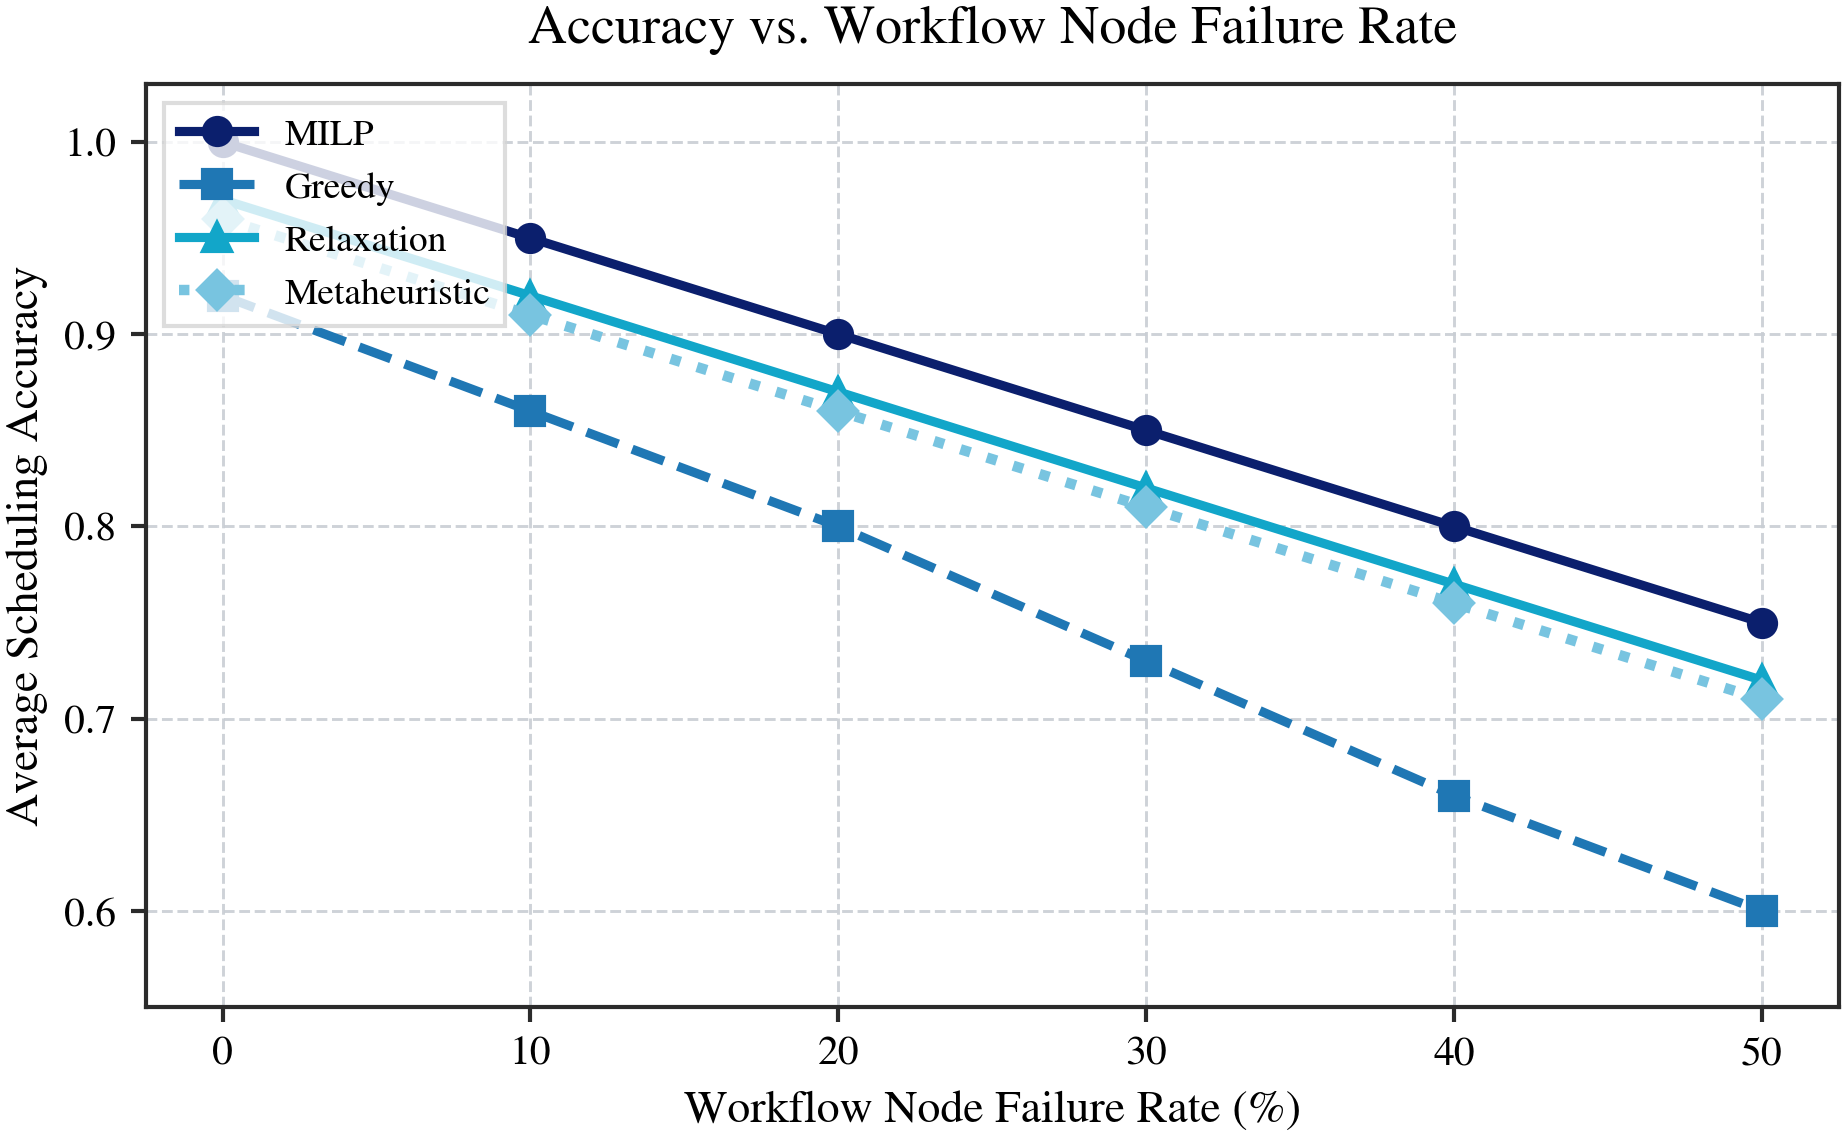
\includegraphics[width=\linewidth]{Figures/perf_failure_accuracy.png}
\caption{Reported average-accuracy comparison under workflow-node failure rates from 0\% to 50\%.}
\label{fig:perf_failure_accuracy}
\end{subfigure}
\caption{Performance comparisons across deadline flexibility, federated resource scale, workflow scale, and workflow-node failure rate.}
\label{fig:performance_comparisons}
\end{figure*}

